% Created by tikzDevice version 0.10.1 on 2017-11-29 19:14:58
% !TEX encoding = UTF-8 Unicode
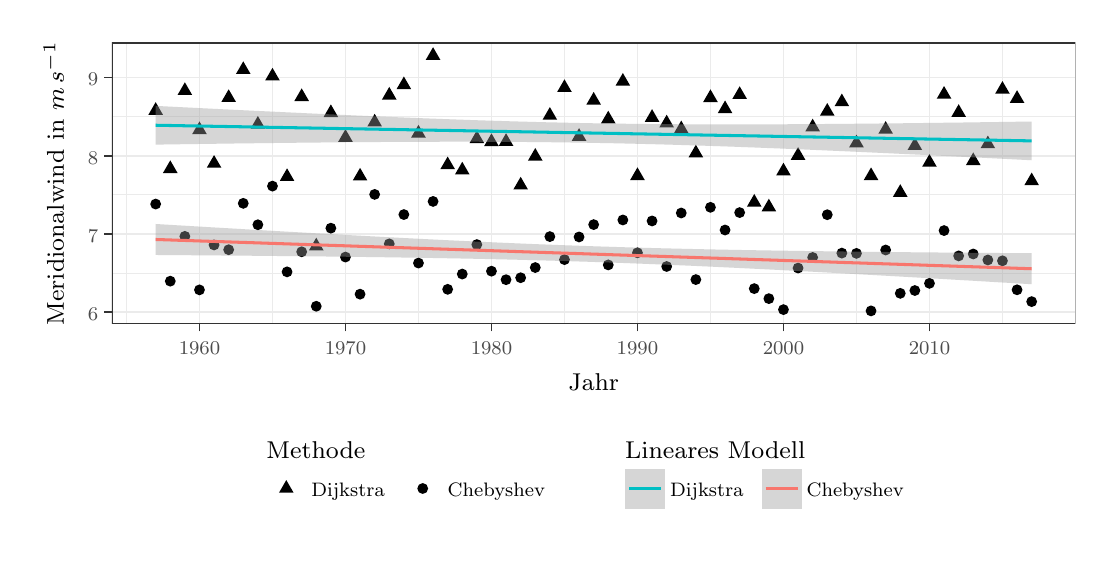
\begin{tikzpicture}[font=\footnotesize,x=1pt,y=1pt]
\definecolor{fillColor}{RGB}{255,255,255}
\path[use as bounding box,fill=fillColor,fill opacity=0.00] (0,0) rectangle (384.11,184.94);
\begin{scope}
\path[clip] (  0.00,  0.00) rectangle (384.11,184.94);
\definecolor{drawColor}{RGB}{255,255,255}
\definecolor{fillColor}{RGB}{255,255,255}

\path[draw=drawColor,line width= 0.6pt,line join=round,line cap=round,fill=fillColor] (  0.00,  0.00) rectangle (384.11,184.94);
\end{scope}
\begin{scope}
\path[clip] ( 30.42, 77.99) rectangle (378.61,179.44);
\definecolor{fillColor}{RGB}{255,255,255}

\path[fill=fillColor] ( 30.42, 77.99) rectangle (378.61,179.44);
\definecolor{drawColor}{gray}{0.92}

\path[draw=drawColor,line width= 0.3pt,line join=round] ( 30.42, 96.26) --
	(378.61, 96.26);

\path[draw=drawColor,line width= 0.3pt,line join=round] ( 30.42,124.54) --
	(378.61,124.54);

\path[draw=drawColor,line width= 0.3pt,line join=round] ( 30.42,152.81) --
	(378.61,152.81);

\path[draw=drawColor,line width= 0.3pt,line join=round] ( 35.70, 77.99) --
	( 35.70,179.44);

\path[draw=drawColor,line width= 0.3pt,line join=round] ( 88.46, 77.99) --
	( 88.46,179.44);

\path[draw=drawColor,line width= 0.3pt,line join=round] (141.21, 77.99) --
	(141.21,179.44);

\path[draw=drawColor,line width= 0.3pt,line join=round] (193.97, 77.99) --
	(193.97,179.44);

\path[draw=drawColor,line width= 0.3pt,line join=round] (246.72, 77.99) --
	(246.72,179.44);

\path[draw=drawColor,line width= 0.3pt,line join=round] (299.48, 77.99) --
	(299.48,179.44);

\path[draw=drawColor,line width= 0.3pt,line join=round] (352.23, 77.99) --
	(352.23,179.44);

\path[draw=drawColor,line width= 0.3pt,line join=round] (378.61, 77.99) --
	(378.61,179.44);

\path[draw=drawColor,line width= 0.6pt,line join=round] ( 30.42, 82.12) --
	(378.61, 82.12);

\path[draw=drawColor,line width= 0.6pt,line join=round] ( 30.42,110.40) --
	(378.61,110.40);

\path[draw=drawColor,line width= 0.6pt,line join=round] ( 30.42,138.67) --
	(378.61,138.67);

\path[draw=drawColor,line width= 0.6pt,line join=round] ( 30.42,166.95) --
	(378.61,166.95);

\path[draw=drawColor,line width= 0.6pt,line join=round] ( 62.08, 77.99) --
	( 62.08,179.44);

\path[draw=drawColor,line width= 0.6pt,line join=round] (114.83, 77.99) --
	(114.83,179.44);

\path[draw=drawColor,line width= 0.6pt,line join=round] (167.59, 77.99) --
	(167.59,179.44);

\path[draw=drawColor,line width= 0.6pt,line join=round] (220.34, 77.99) --
	(220.34,179.44);

\path[draw=drawColor,line width= 0.6pt,line join=round] (273.10, 77.99) --
	(273.10,179.44);

\path[draw=drawColor,line width= 0.6pt,line join=round] (325.86, 77.99) --
	(325.86,179.44);
\definecolor{fillColor}{RGB}{0,0,0}

\path[fill=fillColor] ( 46.25,121.20) circle (  1.96);

\path[fill=fillColor] ( 51.53, 93.34) circle (  1.96);

\path[fill=fillColor] ( 56.80,109.53) circle (  1.96);

\path[fill=fillColor] ( 62.08, 90.19) circle (  1.96);

\path[fill=fillColor] ( 67.35,106.43) circle (  1.96);

\path[fill=fillColor] ( 72.63,104.70) circle (  1.96);

\path[fill=fillColor] ( 77.90,121.46) circle (  1.96);

\path[fill=fillColor] ( 83.18,113.72) circle (  1.96);

\path[fill=fillColor] ( 88.46,127.69) circle (  1.96);

\path[fill=fillColor] ( 93.73, 96.70) circle (  1.96);

\path[fill=fillColor] ( 99.01,103.96) circle (  1.96);

\path[fill=fillColor] (104.28, 84.27) circle (  1.96);

\path[fill=fillColor] (109.56,112.49) circle (  1.96);

\path[fill=fillColor] (114.83,102.05) circle (  1.96);

\path[fill=fillColor] (120.11, 88.64) circle (  1.96);

\path[fill=fillColor] (125.38,124.69) circle (  1.96);

\path[fill=fillColor] (130.66,106.82) circle (  1.96);

\path[fill=fillColor] (135.94,117.41) circle (  1.96);

\path[fill=fillColor] (141.21, 99.88) circle (  1.96);

\path[fill=fillColor] (146.49,122.15) circle (  1.96);

\path[fill=fillColor] (151.76, 90.39) circle (  1.96);

\path[fill=fillColor] (157.04, 95.91) circle (  1.96);

\path[fill=fillColor] (162.31,106.56) circle (  1.96);

\path[fill=fillColor] (167.59, 96.95) circle (  1.96);

\path[fill=fillColor] (172.86, 93.87) circle (  1.96);

\path[fill=fillColor] (178.14, 94.58) circle (  1.96);

\path[fill=fillColor] (183.42, 98.26) circle (  1.96);

\path[fill=fillColor] (188.69,109.44) circle (  1.96);

\path[fill=fillColor] (193.97,101.13) circle (  1.96);

\path[fill=fillColor] (199.24,109.31) circle (  1.96);

\path[fill=fillColor] (204.52,113.78) circle (  1.96);

\path[fill=fillColor] (209.79, 99.21) circle (  1.96);

\path[fill=fillColor] (215.07,115.45) circle (  1.96);

\path[fill=fillColor] (220.34,103.59) circle (  1.96);

\path[fill=fillColor] (225.62,115.10) circle (  1.96);

\path[fill=fillColor] (230.90, 98.64) circle (  1.96);

\path[fill=fillColor] (236.17,117.97) circle (  1.96);

\path[fill=fillColor] (241.45, 93.91) circle (  1.96);

\path[fill=fillColor] (246.72,120.02) circle (  1.96);

\path[fill=fillColor] (252.00,111.82) circle (  1.96);

\path[fill=fillColor] (257.27,118.12) circle (  1.96);

\path[fill=fillColor] (262.55, 90.65) circle (  1.96);

\path[fill=fillColor] (267.83, 87.03) circle (  1.96);

\path[fill=fillColor] (273.10, 83.06) circle (  1.96);

\path[fill=fillColor] (278.38, 98.08) circle (  1.96);

\path[fill=fillColor] (283.65,101.91) circle (  1.96);

\path[fill=fillColor] (288.93,117.35) circle (  1.96);

\path[fill=fillColor] (294.20,103.48) circle (  1.96);

\path[fill=fillColor] (299.48,103.38) circle (  1.96);

\path[fill=fillColor] (304.75, 82.60) circle (  1.96);

\path[fill=fillColor] (310.03,104.60) circle (  1.96);

\path[fill=fillColor] (315.31, 88.94) circle (  1.96);

\path[fill=fillColor] (320.58, 89.96) circle (  1.96);

\path[fill=fillColor] (325.86, 92.55) circle (  1.96);

\path[fill=fillColor] (331.13,111.62) circle (  1.96);

\path[fill=fillColor] (336.41,102.47) circle (  1.96);

\path[fill=fillColor] (341.68,103.16) circle (  1.96);

\path[fill=fillColor] (346.96,100.99) circle (  1.96);

\path[fill=fillColor] (352.23,100.69) circle (  1.96);

\path[fill=fillColor] (357.51, 90.22) circle (  1.96);

\path[fill=fillColor] (362.79, 85.95) circle (  1.96);

\path[fill=fillColor] ( 46.25,158.03) --
	( 48.89,153.45) --
	( 43.61,153.45) --
	cycle;

\path[fill=fillColor] ( 51.53,137.00) --
	( 54.17,132.42) --
	( 48.88,132.42) --
	cycle;

\path[fill=fillColor] ( 56.80,165.21) --
	( 59.44,160.63) --
	( 54.16,160.63) --
	cycle;

\path[fill=fillColor] ( 62.08,151.05) --
	( 64.72,146.47) --
	( 59.44,146.47) --
	cycle;

\path[fill=fillColor] ( 67.35,138.91) --
	( 70.00,134.33) --
	( 64.71,134.33) --
	cycle;

\path[fill=fillColor] ( 72.63,162.68) --
	( 75.27,158.10) --
	( 69.99,158.10) --
	cycle;

\path[fill=fillColor] ( 77.90,172.78) --
	( 80.55,168.20) --
	( 75.26,168.20) --
	cycle;

\path[fill=fillColor] ( 83.18,153.03) --
	( 85.82,148.45) --
	( 80.54,148.45) --
	cycle;

\path[fill=fillColor] ( 88.46,170.43) --
	( 91.10,165.86) --
	( 85.81,165.86) --
	cycle;

\path[fill=fillColor] ( 93.73,134.12) --
	( 96.37,129.54) --
	( 91.09,129.54) --
	cycle;

\path[fill=fillColor] ( 99.01,163.02) --
	(101.65,158.44) --
	( 96.36,158.44) --
	cycle;

\path[fill=fillColor] (104.28,109.05) --
	(106.92,104.47) --
	(101.64,104.47) --
	cycle;

\path[fill=fillColor] (109.56,157.21) --
	(112.20,152.63) --
	(106.92,152.63) --
	cycle;

\path[fill=fillColor] (114.83,148.26) --
	(117.48,143.68) --
	(112.19,143.68) --
	cycle;

\path[fill=fillColor] (120.11,134.29) --
	(122.75,129.72) --
	(117.47,129.72) --
	cycle;

\path[fill=fillColor] (125.38,153.83) --
	(128.03,149.25) --
	(122.74,149.25) --
	cycle;

\path[fill=fillColor] (130.66,163.54) --
	(133.30,158.96) --
	(128.02,158.96) --
	cycle;

\path[fill=fillColor] (135.94,167.31) --
	(138.58,162.73) --
	(133.29,162.73) --
	cycle;

\path[fill=fillColor] (141.21,149.81) --
	(143.85,145.24) --
	(138.57,145.24) --
	cycle;

\path[fill=fillColor] (146.49,177.88) --
	(149.13,173.31) --
	(143.84,173.31) --
	cycle;

\path[fill=fillColor] (151.76,138.38) --
	(154.41,133.81) --
	(149.12,133.81) --
	cycle;

\path[fill=fillColor] (157.04,136.48) --
	(159.68,131.90) --
	(154.40,131.90) --
	cycle;

\path[fill=fillColor] (162.31,147.82) --
	(164.96,143.24) --
	(159.67,143.24) --
	cycle;

\path[fill=fillColor] (167.59,146.74) --
	(170.23,142.16) --
	(164.95,142.16) --
	cycle;

\path[fill=fillColor] (172.86,146.79) --
	(175.51,142.21) --
	(170.22,142.21) --
	cycle;

\path[fill=fillColor] (178.14,131.05) --
	(180.78,126.47) --
	(175.50,126.47) --
	cycle;

\path[fill=fillColor] (183.42,141.46) --
	(186.06,136.89) --
	(180.77,136.89) --
	cycle;

\path[fill=fillColor] (188.69,156.25) --
	(191.33,151.67) --
	(186.05,151.67) --
	cycle;

\path[fill=fillColor] (193.97,166.28) --
	(196.61,161.70) --
	(191.32,161.70) --
	cycle;

\path[fill=fillColor] (199.24,148.63) --
	(201.89,144.05) --
	(196.60,144.05) --
	cycle;

\path[fill=fillColor] (204.52,161.72) --
	(207.16,157.14) --
	(201.88,157.14) --
	cycle;

\path[fill=fillColor] (209.79,154.92) --
	(212.44,150.35) --
	(207.15,150.35) --
	cycle;

\path[fill=fillColor] (215.07,168.56) --
	(217.71,163.98) --
	(212.43,163.98) --
	cycle;

\path[fill=fillColor] (220.34,134.46) --
	(222.99,129.88) --
	(217.70,129.88) --
	cycle;

\path[fill=fillColor] (225.62,155.50) --
	(228.26,150.92) --
	(222.98,150.92) --
	cycle;

\path[fill=fillColor] (230.90,153.48) --
	(233.54,148.90) --
	(228.25,148.90) --
	cycle;

\path[fill=fillColor] (236.17,151.37) --
	(238.81,146.80) --
	(233.53,146.80) --
	cycle;

\path[fill=fillColor] (241.45,142.65) --
	(244.09,138.08) --
	(238.80,138.08) --
	cycle;

\path[fill=fillColor] (246.72,162.64) --
	(249.37,158.06) --
	(244.08,158.06) --
	cycle;

\path[fill=fillColor] (252.00,158.63) --
	(254.64,154.05) --
	(249.36,154.05) --
	cycle;

\path[fill=fillColor] (257.27,163.77) --
	(259.92,159.19) --
	(254.63,159.19) --
	cycle;

\path[fill=fillColor] (262.55,124.85) --
	(265.19,120.27) --
	(259.91,120.27) --
	cycle;

\path[fill=fillColor] (267.83,123.14) --
	(270.47,118.56) --
	(265.18,118.56) --
	cycle;

\path[fill=fillColor] (273.10,136.13) --
	(275.74,131.55) --
	(270.46,131.55) --
	cycle;

\path[fill=fillColor] (278.38,141.77) --
	(281.02,137.20) --
	(275.73,137.20) --
	cycle;

\path[fill=fillColor] (283.65,152.06) --
	(286.29,147.48) --
	(281.01,147.48) --
	cycle;

\path[fill=fillColor] (288.93,157.71) --
	(291.57,153.14) --
	(286.28,153.14) --
	cycle;

\path[fill=fillColor] (294.20,161.13) --
	(296.85,156.55) --
	(291.56,156.55) --
	cycle;

\path[fill=fillColor] (299.48,146.28) --
	(302.12,141.71) --
	(296.84,141.71) --
	cycle;

\path[fill=fillColor] (304.75,134.44) --
	(307.40,129.86) --
	(302.11,129.86) --
	cycle;

\path[fill=fillColor] (310.03,151.19) --
	(312.67,146.61) --
	(307.39,146.61) --
	cycle;

\path[fill=fillColor] (315.31,128.38) --
	(317.95,123.81) --
	(312.66,123.81) --
	cycle;

\path[fill=fillColor] (320.58,145.32) --
	(323.22,140.74) --
	(317.94,140.74) --
	cycle;

\path[fill=fillColor] (325.86,139.27) --
	(328.50,134.69) --
	(323.21,134.69) --
	cycle;

\path[fill=fillColor] (331.13,163.86) --
	(333.77,159.28) --
	(328.49,159.28) --
	cycle;

\path[fill=fillColor] (336.41,157.30) --
	(339.05,152.72) --
	(333.77,152.72) --
	cycle;

\path[fill=fillColor] (341.68,139.86) --
	(344.33,135.28) --
	(339.04,135.28) --
	cycle;

\path[fill=fillColor] (346.96,145.95) --
	(349.60,141.37) --
	(344.32,141.37) --
	cycle;

\path[fill=fillColor] (352.23,165.64) --
	(354.88,161.07) --
	(349.59,161.07) --
	cycle;

\path[fill=fillColor] (357.51,162.34) --
	(360.15,157.77) --
	(354.87,157.77) --
	cycle;

\path[fill=fillColor] (362.79,132.59) --
	(365.43,128.01) --
	(360.14,128.01) --
	cycle;
\definecolor{fillColor}{RGB}{153,153,153}

\path[fill=fillColor,fill opacity=0.40] ( 46.25,114.00) --
	( 50.26,113.76) --
	( 54.26,113.52) --
	( 58.27,113.29) --
	( 62.28,113.05) --
	( 66.28,112.81) --
	( 70.29,112.58) --
	( 74.30,112.35) --
	( 78.31,112.11) --
	( 82.31,111.88) --
	( 86.32,111.65) --
	( 90.33,111.42) --
	( 94.33,111.19) --
	( 98.34,110.97) --
	(102.35,110.74) --
	(106.35,110.52) --
	(110.36,110.30) --
	(114.37,110.08) --
	(118.37,109.86) --
	(122.38,109.64) --
	(126.39,109.43) --
	(130.39,109.22) --
	(134.40,109.01) --
	(138.41,108.80) --
	(142.41,108.60) --
	(146.42,108.40) --
	(150.43,108.20) --
	(154.43,108.01) --
	(158.44,107.82) --
	(162.45,107.63) --
	(166.45,107.45) --
	(170.46,107.27) --
	(174.47,107.10) --
	(178.47,106.93) --
	(182.48,106.76) --
	(186.49,106.61) --
	(190.49,106.45) --
	(194.50,106.30) --
	(198.51,106.16) --
	(202.51,106.02) --
	(206.52,105.88) --
	(210.53,105.76) --
	(214.54,105.63) --
	(218.54,105.51) --
	(222.55,105.40) --
	(226.56,105.29) --
	(230.56,105.19) --
	(234.57,105.09) --
	(238.58,105.00) --
	(242.58,104.91) --
	(246.59,104.82) --
	(250.60,104.74) --
	(254.60,104.66) --
	(258.61,104.59) --
	(262.62,104.52) --
	(266.62,104.45) --
	(270.63,104.39) --
	(274.64,104.33) --
	(278.64,104.27) --
	(282.65,104.21) --
	(286.66,104.16) --
	(290.66,104.11) --
	(294.67,104.06) --
	(298.68,104.01) --
	(302.68,103.96) --
	(306.69,103.92) --
	(310.70,103.88) --
	(314.70,103.83) --
	(318.71,103.79) --
	(322.72,103.76) --
	(326.72,103.72) --
	(330.73,103.68) --
	(334.74,103.65) --
	(338.74,103.62) --
	(342.75,103.58) --
	(346.76,103.55) --
	(350.77,103.52) --
	(354.77,103.49) --
	(358.78,103.46) --
	(362.79,103.43) --
	(362.79, 92.23) --
	(358.78, 92.47) --
	(354.77, 92.71) --
	(350.77, 92.94) --
	(346.76, 93.18) --
	(342.75, 93.42) --
	(338.74, 93.65) --
	(334.74, 93.88) --
	(330.73, 94.12) --
	(326.72, 94.35) --
	(322.72, 94.58) --
	(318.71, 94.81) --
	(314.70, 95.04) --
	(310.70, 95.26) --
	(306.69, 95.49) --
	(302.68, 95.71) --
	(298.68, 95.93) --
	(294.67, 96.15) --
	(290.66, 96.37) --
	(286.66, 96.59) --
	(282.65, 96.80) --
	(278.64, 97.01) --
	(274.64, 97.22) --
	(270.63, 97.43) --
	(266.62, 97.63) --
	(262.62, 97.83) --
	(258.61, 98.03) --
	(254.60, 98.22) --
	(250.60, 98.41) --
	(246.59, 98.60) --
	(242.58, 98.78) --
	(238.58, 98.96) --
	(234.57, 99.13) --
	(230.56, 99.30) --
	(226.56, 99.46) --
	(222.55, 99.62) --
	(218.54, 99.78) --
	(214.54, 99.93) --
	(210.53,100.07) --
	(206.52,100.21) --
	(202.51,100.35) --
	(198.51,100.47) --
	(194.50,100.60) --
	(190.49,100.72) --
	(186.49,100.83) --
	(182.48,100.94) --
	(178.47,101.04) --
	(174.47,101.14) --
	(170.46,101.23) --
	(166.45,101.32) --
	(162.45,101.41) --
	(158.44,101.49) --
	(154.43,101.57) --
	(150.43,101.64) --
	(146.42,101.71) --
	(142.41,101.78) --
	(138.41,101.84) --
	(134.40,101.90) --
	(130.39,101.96) --
	(126.39,102.02) --
	(122.38,102.07) --
	(118.37,102.12) --
	(114.37,102.17) --
	(110.36,102.22) --
	(106.35,102.27) --
	(102.35,102.31) --
	( 98.34,102.35) --
	( 94.33,102.40) --
	( 90.33,102.43) --
	( 86.32,102.47) --
	( 82.31,102.51) --
	( 78.31,102.55) --
	( 74.30,102.58) --
	( 70.29,102.61) --
	( 66.28,102.65) --
	( 62.28,102.68) --
	( 58.27,102.71) --
	( 54.26,102.74) --
	( 50.26,102.77) --
	( 46.25,102.80) --
	cycle;
\definecolor{drawColor}{RGB}{248,118,109}

\path[draw=drawColor,line width= 1.1pt,line join=round] ( 46.25,108.40) --
	( 50.26,108.27) --
	( 54.26,108.13) --
	( 58.27,108.00) --
	( 62.28,107.86) --
	( 66.28,107.73) --
	( 70.29,107.60) --
	( 74.30,107.46) --
	( 78.31,107.33) --
	( 82.31,107.20) --
	( 86.32,107.06) --
	( 90.33,106.93) --
	( 94.33,106.79) --
	( 98.34,106.66) --
	(102.35,106.53) --
	(106.35,106.39) --
	(110.36,106.26) --
	(114.37,106.13) --
	(118.37,105.99) --
	(122.38,105.86) --
	(126.39,105.72) --
	(130.39,105.59) --
	(134.40,105.46) --
	(138.41,105.32) --
	(142.41,105.19) --
	(146.42,105.05) --
	(150.43,104.92) --
	(154.43,104.79) --
	(158.44,104.65) --
	(162.45,104.52) --
	(166.45,104.39) --
	(170.46,104.25) --
	(174.47,104.12) --
	(178.47,103.98) --
	(182.48,103.85) --
	(186.49,103.72) --
	(190.49,103.58) --
	(194.50,103.45) --
	(198.51,103.32) --
	(202.51,103.18) --
	(206.52,103.05) --
	(210.53,102.91) --
	(214.54,102.78) --
	(218.54,102.65) --
	(222.55,102.51) --
	(226.56,102.38) --
	(230.56,102.25) --
	(234.57,102.11) --
	(238.58,101.98) --
	(242.58,101.84) --
	(246.59,101.71) --
	(250.60,101.58) --
	(254.60,101.44) --
	(258.61,101.31) --
	(262.62,101.17) --
	(266.62,101.04) --
	(270.63,100.91) --
	(274.64,100.77) --
	(278.64,100.64) --
	(282.65,100.51) --
	(286.66,100.37) --
	(290.66,100.24) --
	(294.67,100.10) --
	(298.68, 99.97) --
	(302.68, 99.84) --
	(306.69, 99.70) --
	(310.70, 99.57) --
	(314.70, 99.44) --
	(318.71, 99.30) --
	(322.72, 99.17) --
	(326.72, 99.03) --
	(330.73, 98.90) --
	(334.74, 98.77) --
	(338.74, 98.63) --
	(342.75, 98.50) --
	(346.76, 98.37) --
	(350.77, 98.23) --
	(354.77, 98.10) --
	(358.78, 97.96) --
	(362.79, 97.83);

\path[fill=fillColor,fill opacity=0.40] ( 46.25,156.68) --
	( 50.26,156.47) --
	( 54.26,156.27) --
	( 58.27,156.07) --
	( 62.28,155.87) --
	( 66.28,155.67) --
	( 70.29,155.47) --
	( 74.30,155.28) --
	( 78.31,155.08) --
	( 82.31,154.89) --
	( 86.32,154.70) --
	( 90.33,154.51) --
	( 94.33,154.32) --
	( 98.34,154.13) --
	(102.35,153.94) --
	(106.35,153.76) --
	(110.36,153.58) --
	(114.37,153.40) --
	(118.37,153.22) --
	(122.38,153.05) --
	(126.39,152.88) --
	(130.39,152.71) --
	(134.40,152.54) --
	(138.41,152.38) --
	(142.41,152.22) --
	(146.42,152.07) --
	(150.43,151.92) --
	(154.43,151.77) --
	(158.44,151.63) --
	(162.45,151.49) --
	(166.45,151.36) --
	(170.46,151.24) --
	(174.47,151.11) --
	(178.47,151.00) --
	(182.48,150.89) --
	(186.49,150.78) --
	(190.49,150.69) --
	(194.50,150.60) --
	(198.51,150.51) --
	(202.51,150.43) --
	(206.52,150.36) --
	(210.53,150.30) --
	(214.54,150.24) --
	(218.54,150.19) --
	(222.55,150.14) --
	(226.56,150.10) --
	(230.56,150.07) --
	(234.57,150.04) --
	(238.58,150.02) --
	(242.58,150.00) --
	(246.59,149.99) --
	(250.60,149.99) --
	(254.60,149.99) --
	(258.61,149.99) --
	(262.62,150.00) --
	(266.62,150.01) --
	(270.63,150.02) --
	(274.64,150.04) --
	(278.64,150.06) --
	(282.65,150.09) --
	(286.66,150.12) --
	(290.66,150.15) --
	(294.67,150.18) --
	(298.68,150.22) --
	(302.68,150.26) --
	(306.69,150.30) --
	(310.70,150.34) --
	(314.70,150.38) --
	(318.71,150.43) --
	(322.72,150.48) --
	(326.72,150.53) --
	(330.73,150.58) --
	(334.74,150.63) --
	(338.74,150.68) --
	(342.75,150.74) --
	(346.76,150.80) --
	(350.77,150.85) --
	(354.77,150.91) --
	(358.78,150.97) --
	(362.79,151.03) --
	(362.79,137.03) --
	(358.78,137.23) --
	(354.77,137.44) --
	(350.77,137.64) --
	(346.76,137.84) --
	(342.75,138.04) --
	(338.74,138.23) --
	(334.74,138.43) --
	(330.73,138.62) --
	(326.72,138.82) --
	(322.72,139.01) --
	(318.71,139.20) --
	(314.70,139.39) --
	(310.70,139.58) --
	(306.69,139.76) --
	(302.68,139.95) --
	(298.68,140.13) --
	(294.67,140.31) --
	(290.66,140.48) --
	(286.66,140.66) --
	(282.65,140.83) --
	(278.64,141.00) --
	(274.64,141.16) --
	(270.63,141.33) --
	(266.62,141.48) --
	(262.62,141.64) --
	(258.61,141.79) --
	(254.60,141.94) --
	(250.60,142.08) --
	(246.59,142.21) --
	(242.58,142.35) --
	(238.58,142.47) --
	(234.57,142.59) --
	(230.56,142.71) --
	(226.56,142.82) --
	(222.55,142.92) --
	(218.54,143.02) --
	(214.54,143.11) --
	(210.53,143.20) --
	(206.52,143.27) --
	(202.51,143.35) --
	(198.51,143.41) --
	(194.50,143.47) --
	(190.49,143.52) --
	(186.49,143.57) --
	(182.48,143.61) --
	(178.47,143.64) --
	(174.47,143.67) --
	(170.46,143.69) --
	(166.45,143.70) --
	(162.45,143.72) --
	(158.44,143.72) --
	(154.43,143.72) --
	(150.43,143.72) --
	(146.42,143.71) --
	(142.41,143.70) --
	(138.41,143.69) --
	(134.40,143.67) --
	(130.39,143.64) --
	(126.39,143.62) --
	(122.38,143.59) --
	(118.37,143.56) --
	(114.37,143.53) --
	(110.36,143.49) --
	(106.35,143.45) --
	(102.35,143.41) --
	( 98.34,143.37) --
	( 94.33,143.32) --
	( 90.33,143.28) --
	( 86.32,143.23) --
	( 82.31,143.18) --
	( 78.31,143.13) --
	( 74.30,143.08) --
	( 70.29,143.02) --
	( 66.28,142.97) --
	( 62.28,142.91) --
	( 58.27,142.86) --
	( 54.26,142.80) --
	( 50.26,142.74) --
	( 46.25,142.68) --
	cycle;
\definecolor{drawColor}{RGB}{0,191,196}

\path[draw=drawColor,line width= 1.1pt,line join=round] ( 46.25,149.68) --
	( 50.26,149.61) --
	( 54.26,149.54) --
	( 58.27,149.46) --
	( 62.28,149.39) --
	( 66.28,149.32) --
	( 70.29,149.25) --
	( 74.30,149.18) --
	( 78.31,149.11) --
	( 82.31,149.03) --
	( 86.32,148.96) --
	( 90.33,148.89) --
	( 94.33,148.82) --
	( 98.34,148.75) --
	(102.35,148.68) --
	(106.35,148.61) --
	(110.36,148.53) --
	(114.37,148.46) --
	(118.37,148.39) --
	(122.38,148.32) --
	(126.39,148.25) --
	(130.39,148.18) --
	(134.40,148.11) --
	(138.41,148.03) --
	(142.41,147.96) --
	(146.42,147.89) --
	(150.43,147.82) --
	(154.43,147.75) --
	(158.44,147.68) --
	(162.45,147.60) --
	(166.45,147.53) --
	(170.46,147.46) --
	(174.47,147.39) --
	(178.47,147.32) --
	(182.48,147.25) --
	(186.49,147.18) --
	(190.49,147.10) --
	(194.50,147.03) --
	(198.51,146.96) --
	(202.51,146.89) --
	(206.52,146.82) --
	(210.53,146.75) --
	(214.54,146.68) --
	(218.54,146.60) --
	(222.55,146.53) --
	(226.56,146.46) --
	(230.56,146.39) --
	(234.57,146.32) --
	(238.58,146.25) --
	(242.58,146.17) --
	(246.59,146.10) --
	(250.60,146.03) --
	(254.60,145.96) --
	(258.61,145.89) --
	(262.62,145.82) --
	(266.62,145.75) --
	(270.63,145.67) --
	(274.64,145.60) --
	(278.64,145.53) --
	(282.65,145.46) --
	(286.66,145.39) --
	(290.66,145.32) --
	(294.67,145.25) --
	(298.68,145.17) --
	(302.68,145.10) --
	(306.69,145.03) --
	(310.70,144.96) --
	(314.70,144.89) --
	(318.71,144.82) --
	(322.72,144.74) --
	(326.72,144.67) --
	(330.73,144.60) --
	(334.74,144.53) --
	(338.74,144.46) --
	(342.75,144.39) --
	(346.76,144.32) --
	(350.77,144.24) --
	(354.77,144.17) --
	(358.78,144.10) --
	(362.79,144.03);
\definecolor{drawColor}{gray}{0.20}

\path[draw=drawColor,line width= 0.6pt,line join=round,line cap=round] ( 30.42, 77.99) rectangle (378.61,179.44);
\end{scope}
\begin{scope}
\path[clip] (  0.00,  0.00) rectangle (384.11,184.94);
\definecolor{drawColor}{gray}{0.30}

\node[text=drawColor,anchor=base east,inner sep=0pt, outer sep=0pt, scale=  0.88] at ( 25.47, 79.09) {6};

\node[text=drawColor,anchor=base east,inner sep=0pt, outer sep=0pt, scale=  0.88] at ( 25.47,107.37) {7};

\node[text=drawColor,anchor=base east,inner sep=0pt, outer sep=0pt, scale=  0.88] at ( 25.47,135.64) {8};

\node[text=drawColor,anchor=base east,inner sep=0pt, outer sep=0pt, scale=  0.88] at ( 25.47,163.92) {9};
\end{scope}
\begin{scope}
\path[clip] (  0.00,  0.00) rectangle (384.11,184.94);
\definecolor{drawColor}{gray}{0.20}

\path[draw=drawColor,line width= 0.6pt,line join=round] ( 27.67, 82.12) --
	( 30.42, 82.12);

\path[draw=drawColor,line width= 0.6pt,line join=round] ( 27.67,110.40) --
	( 30.42,110.40);

\path[draw=drawColor,line width= 0.6pt,line join=round] ( 27.67,138.67) --
	( 30.42,138.67);

\path[draw=drawColor,line width= 0.6pt,line join=round] ( 27.67,166.95) --
	( 30.42,166.95);
\end{scope}
\begin{scope}
\path[clip] (  0.00,  0.00) rectangle (384.11,184.94);
\definecolor{drawColor}{gray}{0.20}

\path[draw=drawColor,line width= 0.6pt,line join=round] ( 62.08, 75.24) --
	( 62.08, 77.99);

\path[draw=drawColor,line width= 0.6pt,line join=round] (114.83, 75.24) --
	(114.83, 77.99);

\path[draw=drawColor,line width= 0.6pt,line join=round] (167.59, 75.24) --
	(167.59, 77.99);

\path[draw=drawColor,line width= 0.6pt,line join=round] (220.34, 75.24) --
	(220.34, 77.99);

\path[draw=drawColor,line width= 0.6pt,line join=round] (273.10, 75.24) --
	(273.10, 77.99);

\path[draw=drawColor,line width= 0.6pt,line join=round] (325.86, 75.24) --
	(325.86, 77.99);
\end{scope}
\begin{scope}
\path[clip] (  0.00,  0.00) rectangle (384.11,184.94);
\definecolor{drawColor}{gray}{0.30}

\node[text=drawColor,anchor=base,inner sep=0pt, outer sep=0pt, scale=  0.88] at ( 62.08, 66.98) {1960};

\node[text=drawColor,anchor=base,inner sep=0pt, outer sep=0pt, scale=  0.88] at (114.83, 66.98) {1970};

\node[text=drawColor,anchor=base,inner sep=0pt, outer sep=0pt, scale=  0.88] at (167.59, 66.98) {1980};

\node[text=drawColor,anchor=base,inner sep=0pt, outer sep=0pt, scale=  0.88] at (220.34, 66.98) {1990};

\node[text=drawColor,anchor=base,inner sep=0pt, outer sep=0pt, scale=  0.88] at (273.10, 66.98) {2000};

\node[text=drawColor,anchor=base,inner sep=0pt, outer sep=0pt, scale=  0.88] at (325.86, 66.98) {2010};
\end{scope}
\begin{scope}
\path[clip] (  0.00,  0.00) rectangle (384.11,184.94);
\definecolor{drawColor}{RGB}{0,0,0}

\node[text=drawColor,anchor=base,inner sep=0pt, outer sep=0pt, scale=  1.10] at (204.52, 53.91) {Jahr};
\end{scope}
\begin{scope}
\path[clip] (  0.00,  0.00) rectangle (384.11,184.94);
\definecolor{drawColor}{RGB}{0,0,0}

\node[text=drawColor,rotate= 90.00,anchor=base,inner sep=0pt, outer sep=0pt, scale=  1.10] at ( 13.08,128.72) {Meridionalwind in $m\,s^{-1}$};
\end{scope}
\begin{scope}
\path[clip] (  0.00,  0.00) rectangle (384.11,184.94);
\definecolor{fillColor}{RGB}{255,255,255}

\path[fill=fillColor] ( 80.54,  5.50) rectangle (198.83, 42.52);
\end{scope}
\begin{scope}
\path[clip] (  0.00,  0.00) rectangle (384.11,184.94);
\definecolor{drawColor}{RGB}{0,0,0}

\node[text=drawColor,anchor=base west,inner sep=0pt, outer sep=0pt, scale=  1.10] at ( 86.23, 29.26) {Methode};
\end{scope}
\begin{scope}
\path[clip] (  0.00,  0.00) rectangle (384.11,184.94);
\definecolor{fillColor}{RGB}{255,255,255}

\path[fill=fillColor] ( 86.23, 11.19) rectangle (100.68, 25.64);
\end{scope}
\begin{scope}
\path[clip] (  0.00,  0.00) rectangle (384.11,184.94);
\definecolor{fillColor}{RGB}{0,0,0}

\path[fill=fillColor] ( 93.45, 21.47) --
	( 96.10, 16.89) --
	( 90.81, 16.89) --
	cycle;
\end{scope}
\begin{scope}
\path[clip] (  0.00,  0.00) rectangle (384.11,184.94);
\definecolor{fillColor}{RGB}{255,255,255}

\path[fill=fillColor] (135.53, 11.19) rectangle (149.98, 25.64);
\end{scope}
\begin{scope}
\path[clip] (  0.00,  0.00) rectangle (384.11,184.94);
\definecolor{fillColor}{RGB}{0,0,0}

\path[fill=fillColor] (142.75, 18.42) circle (  1.96);
\end{scope}
\begin{scope}
\path[clip] (  0.00,  0.00) rectangle (384.11,184.94);
\definecolor{drawColor}{RGB}{0,0,0}

\node[text=drawColor,anchor=base west,inner sep=0pt, outer sep=0pt, scale=  0.88] at (102.49, 15.39) {Dijkstra};
\end{scope}
\begin{scope}
\path[clip] (  0.00,  0.00) rectangle (384.11,184.94);
\definecolor{drawColor}{RGB}{0,0,0}

\node[text=drawColor,anchor=base west,inner sep=0pt, outer sep=0pt, scale=  0.88] at (151.79, 15.39) {Chebyshev};
\end{scope}
\begin{scope}
\path[clip] (  0.00,  0.00) rectangle (384.11,184.94);
\definecolor{fillColor}{RGB}{255,255,255}

\path[fill=fillColor] (210.21,  5.50) rectangle (328.50, 42.52);
\end{scope}
\begin{scope}
\path[clip] (  0.00,  0.00) rectangle (384.11,184.94);
\definecolor{drawColor}{RGB}{0,0,0}

\node[text=drawColor,anchor=base west,inner sep=0pt, outer sep=0pt, scale=  1.10] at (215.90, 29.26) {Lineares Modell};
\end{scope}
\begin{scope}
\path[clip] (  0.00,  0.00) rectangle (384.11,184.94);
\definecolor{fillColor}{RGB}{255,255,255}

\path[fill=fillColor] (215.90, 11.19) rectangle (230.35, 25.64);
\end{scope}
\begin{scope}
\path[clip] (  0.00,  0.00) rectangle (384.11,184.94);
\definecolor{fillColor}{RGB}{153,153,153}

\path[fill=fillColor,fill opacity=0.40] (215.90, 11.19) rectangle (230.35, 25.64);
\definecolor{drawColor}{RGB}{0,191,196}

\path[draw=drawColor,line width= 1.1pt,line join=round] (217.34, 18.42) -- (228.91, 18.42);
\end{scope}
\begin{scope}
\path[clip] (  0.00,  0.00) rectangle (384.11,184.94);
\definecolor{fillColor}{RGB}{255,255,255}

\path[fill=fillColor] (265.20, 11.19) rectangle (279.65, 25.64);
\end{scope}
\begin{scope}
\path[clip] (  0.00,  0.00) rectangle (384.11,184.94);
\definecolor{fillColor}{RGB}{153,153,153}

\path[fill=fillColor,fill opacity=0.40] (265.20, 11.19) rectangle (279.65, 25.64);
\definecolor{drawColor}{RGB}{248,118,109}

\path[draw=drawColor,line width= 1.1pt,line join=round] (266.64, 18.42) -- (278.21, 18.42);
\end{scope}
\begin{scope}
\path[clip] (  0.00,  0.00) rectangle (384.11,184.94);
\definecolor{drawColor}{RGB}{0,0,0}

\node[text=drawColor,anchor=base west,inner sep=0pt, outer sep=0pt, scale=  0.88] at (232.16, 15.39) {Dijkstra};
\end{scope}
\begin{scope}
\path[clip] (  0.00,  0.00) rectangle (384.11,184.94);
\definecolor{drawColor}{RGB}{0,0,0}

\node[text=drawColor,anchor=base west,inner sep=0pt, outer sep=0pt, scale=  0.88] at (281.46, 15.39) {Chebyshev};
\end{scope}
\end{tikzpicture}
